% =====================================================================
%  Aprendizaje No Supervisado — Unidad 1: Algoritmos de agrupamiento
%  Sesiones 2 a 6 de la planeación didáctica
%  Compilar con: latexmk -pdf Unidad1-Agrupamiento.tex
%  Las figuras se regeneran con: python3 figuras/generar_figuras.py
% =====================================================================
\documentclass[aspectratio=169,11pt]{beamer}

% ---------- Idioma y codificación ----------
\usepackage[utf8]{inputenc}
\usepackage[T1]{fontenc}
\usepackage[spanish,es-noshorthands,es-nodecimaldot]{babel}

% ---------- Paquetes ----------
\usepackage{amsmath,amssymb,bm}
\usepackage{booktabs,array}
\usepackage{listings}
\usepackage{tikz}
\usetikzlibrary{positioning,arrows.meta,calc}
\graphicspath{{figuras/}}

% ---------- Tema y colores (comunes a las presentaciones del curso) ----------
\usetheme{Madrid}
\usefonttheme{professionalfonts}
\definecolor{marino}{HTML}{1F3864}
\definecolor{azul}{HTML}{2E75B6}
\definecolor{naranja}{HTML}{E07B22}
\definecolor{verde}{HTML}{5B9A3C}
\definecolor{fondocod}{HTML}{F4F6F9}
\setbeamercolor{palette primary}{bg=marino,fg=white}
\setbeamercolor{palette secondary}{bg=azul,fg=white}
\setbeamercolor{palette tertiary}{bg=marino,fg=white}
\setbeamercolor{frametitle}{bg=marino,fg=white}
\setbeamercolor{title}{bg=marino,fg=white}
\setbeamercolor{structure}{fg=azul}
\setbeamercolor{block title}{bg=azul,fg=white}
\setbeamercolor{block body}{bg=azul!8}
\setbeamercolor{block title alerted}{bg=naranja,fg=white}
\setbeamercolor{block body alerted}{bg=naranja!10}
\setbeamercolor{block title example}{bg=verde,fg=white}
\setbeamercolor{block body example}{bg=verde!10}
\setbeamercolor{alerted text}{fg=naranja}
\setbeamertemplate{navigation symbols}{}
\setbeamertemplate{itemize items}[circle]
\setbeamertemplate{blocks}[rounded][shadow=false]

\AtBeginSection[]{
  \begin{frame}
    \vfill\centering
    \begin{beamercolorbox}[sep=12pt,center,rounded=true]{title}
      \usebeamerfont{title}\insertsectionhead
    \end{beamercolorbox}
    \vfill
  \end{frame}
}

% Estilo para los diagramas de flujo
\tikzset{
  caja/.style={draw=azul,fill=azul!10,rounded corners,align=center,font=\small,minimum height=9mm},
  flecha/.style={-{Stealth},thick,marino}
}

% ---------- Código ----------
\lstdefinestyle{py}{
  language=Python,
  basicstyle=\ttfamily\scriptsize,
  keywordstyle=\color{marino}\bfseries,
  commentstyle=\color{gray}\itshape,
  stringstyle=\color{naranja},
  backgroundcolor=\color{fondocod},
  frame=single, rulecolor=\color{azul!40},
  showstringspaces=false, columns=fullflexible,
  breaklines=true, xleftmargin=4pt, xrightmargin=4pt
}
\lstset{style=py}

% ---------- Notación ----------
\newcommand{\R}{\mathbb{R}}
\newcommand{\x}{\bm{x}}
\newcommand{\muv}{\bm{\mu}}
\newcommand{\E}{\mathbb{E}}
\newcommand{\N}{\mathcal{N}}

% ---------- Datos de la presentación ----------
\title[Unidad 1: Algoritmos de agrupamiento]{Unidad 1: Algoritmos de agrupamiento}
\subtitle{Aprendizaje No Supervisado}
\author[A. Espinosa Romero]{Arturo Espinosa Romero}
\institute[FMAT]{Maestría en Inteligencia Artificial \\ Facultad de Matemáticas}
\date{Sesiones 2--6}

% =====================================================================
\begin{document}

\begin{frame}
  \titlepage
\end{frame}

\begin{frame}{Mapa de la unidad}
  \begin{columns}[T]
    \column{0.55\textwidth}
    \begin{enumerate}
      \item[\textbf{S2}] k-medias (\emph{k-means})
      \item[\textbf{S3}] Agrupamiento jerárquico
      \item[\textbf{S4}] Modelos de mezclas gaussianas (GMM)
      \item[\textbf{S5}] Agrupamiento por densidad y espectral
      \item[\textbf{S6}] Validación e interpretación de agrupamientos
    \end{enumerate}
    \column{0.42\textwidth}
    \begin{block}{Entregables}
      \begin{itemize}
        \item Laboratorios de S2 a S5
        \item Miniproyecto 1 (S6), 30\,\% de la calificación
      \end{itemize}
    \end{block}
  \end{columns}
  \vspace{6pt}
  \begin{alertblock}{Objetivo de la unidad}
    Construir, comparar y validar modelos de agrupamiento, y comunicar qué
    significan los grupos encontrados para la toma de decisiones.
  \end{alertblock}
\end{frame}

% =====================================================================
\section{El problema del agrupamiento}
% =====================================================================

\begin{frame}{¿Qué es agrupar?}
  Dado $\{\x_1,\dots,\x_n\}\subset\R^d$ sin etiquetas, encontrar una partición (o una
  jerarquía, o asignaciones probabilísticas) en la que los objetos de un mismo grupo
  sean \alert{parecidos} entre sí y \alert{distintos} de los de otros grupos.
  \vspace{6pt}
  \begin{columns}[T]
    \column{0.48\textwidth}
    \begin{block}{Aplicaciones}
      \begin{itemize}
        \item Segmentación de clientes
        \item Tipologías de hogares o municipios
        \item Agrupar documentos por tema
        \item Compresión (cuantización vectorial)
      \end{itemize}
    \end{block}
    \column{0.48\textwidth}
    \begin{alertblock}{¿Qué es un ``grupo''?}
      No hay una única definición. Cada algoritmo asume una:
      \begin{itemize}
        \item cercanía a un centro (k-medias),
        \item conectividad (jerárquico, espectral),
        \item un componente de una distribución (GMM),
        \item una región densa (DBSCAN).
      \end{itemize}
    \end{alertblock}
  \end{columns}
\end{frame}

\begin{frame}{Familias de algoritmos}
  \centering
  \renewcommand{\arraystretch}{1.25}
  \begin{tabular}{@{}llll@{}}
    \toprule
    \textbf{Familia} & \textbf{Algoritmo} & \textbf{Salida} & \textbf{Sesión}\\
    \midrule
    Basada en prototipos & k-medias, k-medoides & Partición plana & S2 \\
    Jerárquica           & Aglomerativo, divisivo & Árbol (dendrograma) & S3 \\
    Basada en modelos    & Mezclas gaussianas & Asignación probabilística & S4 \\
    Basada en densidad   & DBSCAN, HDBSCAN, OPTICS & Partición + ruido & S5 \\
    Basada en grafos     & Agrupamiento espectral & Partición plana & S5 \\
    \bottomrule
  \end{tabular}
  \vspace{8pt}
  \begin{block}{Recordatorio de la Sesión 1}
    El resultado depende del \textbf{preprocesamiento} (escala, valores faltantes) y de la
    \textbf{medida de distancia}. Siempre estandarizar cuando las unidades difieren.
  \end{block}
\end{frame}

% =====================================================================
\section{Sesión 2: k-medias}
% =====================================================================

\begin{frame}{Función objetivo}
  Buscar $k$ centros $\muv_1,\dots,\muv_k$ y una asignación $z_i\in\{1,\dots,k\}$ que minimicen la
  \alert{inercia} (suma de cuadrados dentro de los grupos):
  \[
    J = \sum_{i=1}^{n} \lVert \x_i - \muv_{z_i} \rVert^2
      = \sum_{j=1}^{k}\sum_{i\,:\,z_i=j} \lVert \x_i - \muv_j \rVert^2 .
  \]
  \begin{itemize}
    \item Encontrar el mínimo global es NP-difícil.
    \item Para asignaciones fijas, el centro óptimo es la media del grupo:
          $\muv_j = \frac{1}{n_j}\sum_{i:z_i=j}\x_i$.
    \item Para centros fijos, la asignación óptima es el centro más cercano.
  \end{itemize}
  \begin{block}{Idea}
    Alternar ambos pasos: es un descenso por coordenadas sobre $J$.
  \end{block}
\end{frame}

\begin{frame}{Algoritmo de Lloyd}
  \begin{columns}[c]
    \column{0.45\textwidth}
    \begin{enumerate}
      \item Inicializar $\muv_1,\dots,\muv_k$.
      \item \textbf{Asignación}: $z_i \leftarrow \arg\min_j \lVert\x_i-\muv_j\rVert^2$.
      \item \textbf{Actualización}: $\muv_j \leftarrow$ media de los puntos con $z_i=j$.
      \item Repetir 2--3 hasta que las asignaciones no cambien.
    \end{enumerate}
    \vspace{4pt}
    \begin{itemize}
      \item $J$ nunca aumenta: converge en un número finito de pasos.
      \item Converge a un \alert{mínimo local}.
      \item Costo por iteración: $O(nkd)$.
    \end{itemize}
    \column{0.53\textwidth}
    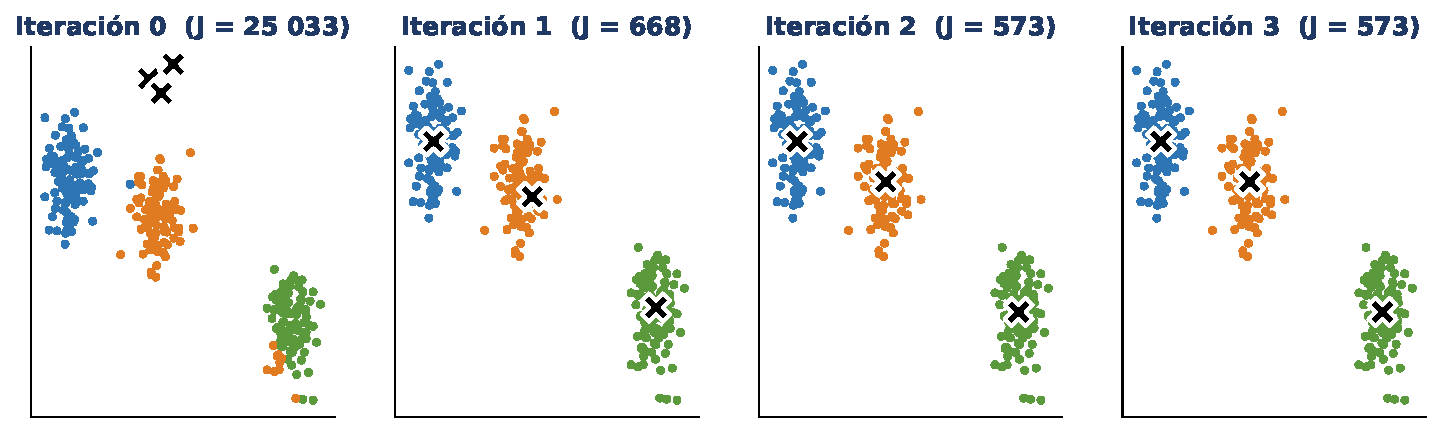
\includegraphics[width=\textwidth]{lloyd_iteraciones}\\
    {\scriptsize Una mala inicialización (cruces arriba) se corrige en pocas iteraciones.}
  \end{columns}
\end{frame}

\begin{frame}{Inicialización: k-means++}
  \begin{columns}[c]
    \column{0.5\textwidth}
    \small
    \begin{enumerate}
      \item Elegir el primer centro al azar entre los datos.
      \item Elegir cada nuevo centro entre los datos con probabilidad
            \[ P(\x_i) = \frac{D(\x_i)^2}{\sum_l D(\x_l)^2}, \]
            donde $D(\x)$ es la distancia al centro ya elegido más cercano.
      \item Ejecutar Lloyd desde esos centros.
    \end{enumerate}
    \vspace{4pt}
    \begin{itemize}
      \item Garantía: en esperanza, $O(\log k)$ veces el óptimo.
      \item En la práctica: \alert{varios reinicios} (\texttt{n\_init}) y quedarse con el menor $J$.
    \end{itemize}
    \column{0.48\textwidth}
    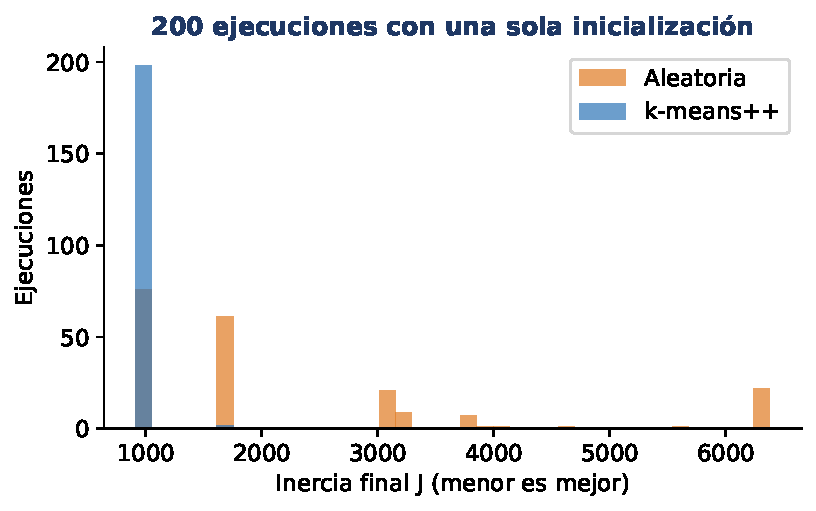
\includegraphics[width=\textwidth]{inicializacion}
  \end{columns}
\end{frame}

\begin{frame}{Elección de $k$}
  \centering
  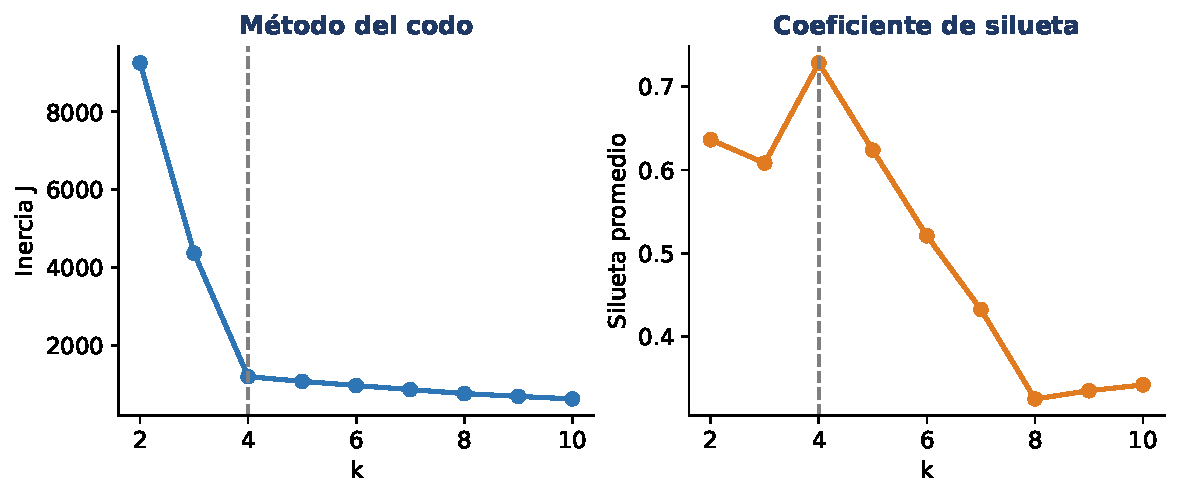
\includegraphics[width=0.7\textwidth]{codo_silueta}
  \small
  \begin{itemize}
    \item \textbf{Codo}: $J$ siempre baja al aumentar $k$; buscar donde la mejora se vuelve marginal.
    \item \textbf{Silueta}: para cada punto, $s(i) = \dfrac{b(i)-a(i)}{\max\{a(i),b(i)\}}\in[-1,1]$, con
          $a(i)$ la distancia media a su grupo y $b(i)$ la del grupo vecino más cercano. Elegir el $k$ con mayor promedio.
    \item El conocimiento del dominio y el uso final también cuentan (más detalle en S6).
  \end{itemize}
\end{frame}

\begin{frame}{Limitaciones de k-medias}
  \centering
  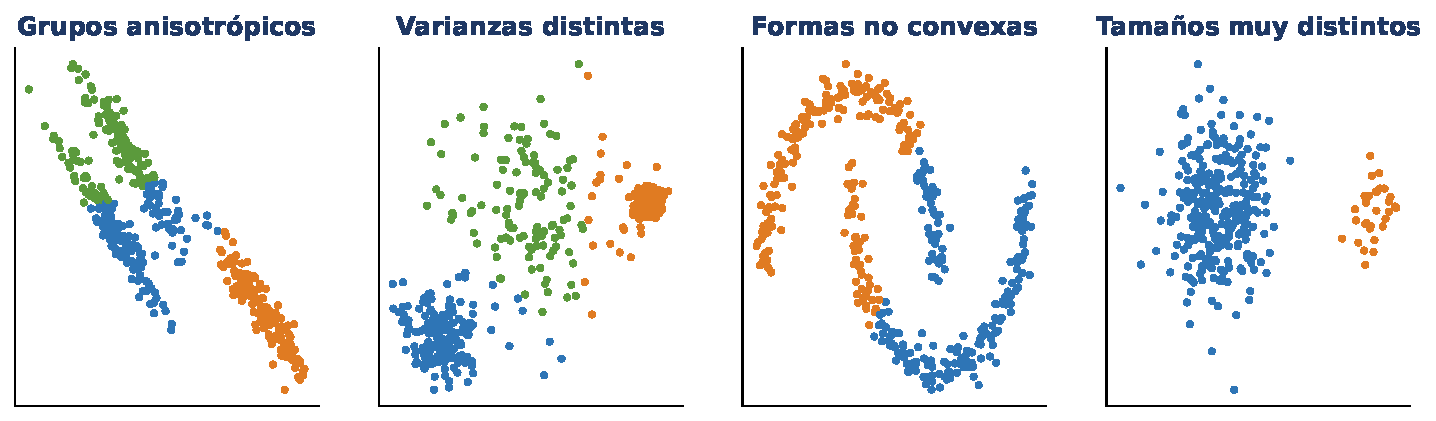
\includegraphics[width=\textwidth]{limitaciones_kmeans}
  \begin{columns}[T]
    \column{0.48\textwidth}
    \begin{itemize}
      \item Supone grupos \alert{esféricos} y de tamaño parecido.
      \item Sensible a la \alert{escala} de las variables.
    \end{itemize}
    \column{0.48\textwidth}
    \begin{itemize}
      \item Sensible a valores \alert{atípicos} (la media lo es).
      \item Hay que fijar $k$; siempre asigna todos los puntos.
    \end{itemize}
  \end{columns}
\end{frame}

\begin{frame}{Variantes}
  \renewcommand{\arraystretch}{1.3}
  \begin{tabular}{@{}>{\raggedright\arraybackslash}p{0.24\textwidth}>{\raggedright\arraybackslash}p{0.4\textwidth}>{\raggedright\arraybackslash}p{0.28\textwidth}@{}}
    \toprule
    \textbf{Variante} & \textbf{Idea} & \textbf{Cuándo usarla}\\
    \midrule
    k-medoides (PAM) & Centros restringidos a observaciones; admite cualquier distancia & Atípicos, distancias no euclidianas \\
    Mini-batch k-medias & Actualiza con lotes pequeños & $n$ muy grande \\
    k-medianas & Usa la mediana y la distancia $\ell_1$ & Robustez \\
    k-modos / k-prototipos & Modas para variables categóricas & Datos categóricos o mixtos \\
    \bottomrule
  \end{tabular}
  \vspace{6pt}
  {\small En scikit-learn: \texttt{KMeans}, \texttt{MiniBatchKMeans}; k-medoides en \texttt{scikit-learn-extra}.}
\end{frame}

\begin{frame}[fragile]{Laboratorio S2: k-medias desde cero}
\begin{lstlisting}
import numpy as np

def kmedias(X, k, max_iter=100, semilla=0):
    rng = np.random.default_rng(semilla)
    C = X[rng.choice(len(X), k, replace=False)]           # inicializacion aleatoria
    for _ in range(max_iter):
        d = ((X[:, None, :] - C[None, :, :])**2).sum(-1)  # distancias n x k
        z = d.argmin(axis=1)                              # paso de asignacion
        C_nuevo = np.array([X[z == j].mean(axis=0) if np.any(z == j) else C[j]
                            for j in range(k)])           # paso de actualizacion
        if np.allclose(C, C_nuevo):
            break
        C = C_nuevo
    inercia = ((X - C[z])**2).sum()
    return z, C, inercia
\end{lstlisting}
  {\small Ejercicio: agregar la inicialización k-means++ y varios reinicios; comparar con \texttt{sklearn.cluster.KMeans}.}
\end{frame}

\begin{frame}[fragile]{Laboratorio S2: segmentación de clientes}
\begin{lstlisting}
import numpy as np, pandas as pd
from sklearn.pipeline import make_pipeline
from sklearn.preprocessing import FunctionTransformer, StandardScaler
from sklearn.cluster import KMeans
from sklearn.metrics import silhouette_score

# UCI Wholesale customers: gasto anual por categoria de 440 clientes
url = ("https://archive.ics.uci.edu/ml/machine-learning-databases/"
       "00292/Wholesale%20customers%20data.csv")
df = pd.read_csv(url).drop(columns=["Channel", "Region"])

prep = make_pipeline(FunctionTransformer(np.log1p), StandardScaler())  # sesgo y escala
X = prep.fit_transform(df)

for k in range(2, 9):
    km = KMeans(k, n_init=10, random_state=0).fit(X)
    print(k, round(km.inertia_, 1), round(silhouette_score(X, km.labels_), 3))

km = KMeans(3, n_init=10, random_state=0).fit(X)
print(df.groupby(km.labels_).median())       # perfil de cada segmento
\end{lstlisting}
\end{frame}

% =====================================================================
\section{Sesión 3: Agrupamiento jerárquico}
% =====================================================================

\begin{frame}{Idea}
  Construir una \alert{jerarquía} de grupos anidados en lugar de una sola partición.
  \vspace{4pt}
  \begin{columns}[T]
    \column{0.48\textwidth}
    \begin{block}{Aglomerativo (de abajo hacia arriba)}
      \begin{enumerate}
        \item Cada punto es un grupo.
        \item Fusionar los dos grupos más cercanos.
        \item Repetir hasta tener un solo grupo.
      \end{enumerate}
    \end{block}
    \column{0.48\textwidth}
    \begin{block}{Divisivo (de arriba hacia abajo)}
      \begin{enumerate}
        \item Todos los puntos en un grupo.
        \item Dividir el grupo menos homogéneo (p.\ ej., con 2-medias).
        \item Repetir hasta tener grupos unitarios.
      \end{enumerate}
    \end{block}
  \end{columns}
  \vspace{6pt}
  \begin{itemize}
    \item No requiere fijar $k$ de antemano: se elige al \textbf{cortar} el árbol.
    \item El aglomerativo es el más usado; la clave es cómo medir la distancia \emph{entre grupos}.
  \end{itemize}
\end{frame}

\begin{frame}{Criterios de enlace}
  Distancia entre los grupos $A$ y $B$:
  \renewcommand{\arraystretch}{1.6}
  \begin{tabular}{@{}lll@{}}
    \toprule
    \textbf{Enlace} & \textbf{Definición} & \textbf{Comportamiento}\\
    \midrule
    Simple   & $\displaystyle\min_{a\in A,\,b\in B} d(a,b)$ & Formas alargadas; efecto \alert{cadena} \\
    Completo & $\displaystyle\max_{a\in A,\,b\in B} d(a,b)$ & Grupos compactos; sensible a atípicos \\
    Promedio & $\displaystyle\frac{1}{|A||B|}\sum_{a\in A}\sum_{b\in B} d(a,b)$ & Intermedio \\
    Ward     & $\displaystyle\frac{|A||B|}{|A|+|B|}\lVert\muv_A-\muv_B\rVert^2$ & Aumento mínimo de la inercia; parecido a k-medias \\
    \bottomrule
  \end{tabular}
  \vspace{4pt}
  {\small Ward requiere distancia euclidiana; los demás admiten cualquier disimilitud.}
\end{frame}

\begin{frame}{El efecto del enlace}
  \centering
  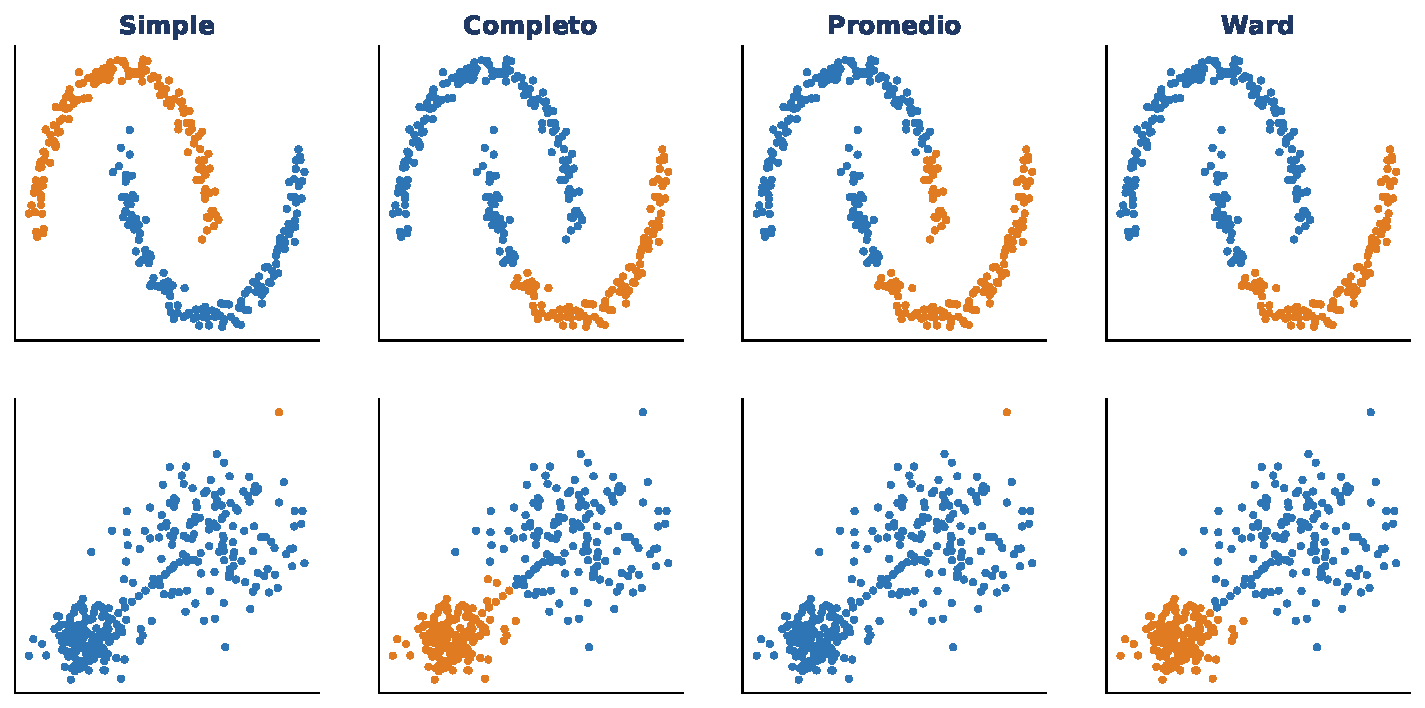
\includegraphics[width=0.85\textwidth]{enlaces}
  \begin{itemize}
    \item Arriba: el enlace simple recupera las lunas; Ward y completo las cortan.
    \item Abajo: un ``puente'' de pocos puntos hace que el enlace simple encadene los dos grupos.
  \end{itemize}
\end{frame}

\begin{frame}{Dendrogramas}
  \centering
  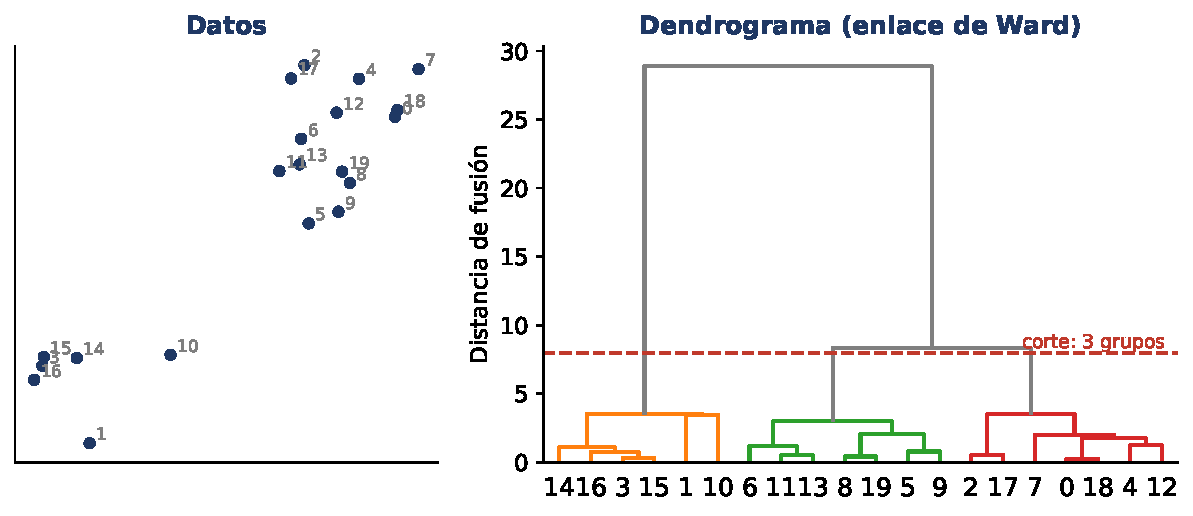
\includegraphics[width=0.85\textwidth]{dendrograma}
  \begin{itemize}
    \item La altura de cada fusión es la distancia entre los grupos fusionados.
    \item \textbf{Cortar} a una altura da una partición; un salto grande sugiere un buen corte.
    \item \textbf{Correlación cofenética}: qué tan bien preserva el árbol las distancias originales.
  \end{itemize}
\end{frame}

\begin{frame}{Complejidad y escalabilidad}
  \begin{itemize}
    \item Requiere la matriz de distancias: memoria $O(n^2)$.
    \item Tiempo $O(n^2\log n)$ en general; $O(n^2)$ para enlace simple (SLINK).
    \item Con $n = 50\,000$ la matriz ocupa $\approx 10$ GB en doble precisión.
  \end{itemize}
  \vspace{4pt}
  \begin{exampleblock}{Estrategias}
    \begin{itemize}
      \item Restringir fusiones a vecinos (\texttt{connectivity} en scikit-learn).
      \item Agrupar primero con k-medias en muchos grupos pequeños y luego jerarquizar los centros.
      \item BIRCH: resume los datos en un árbol de características.
    \end{itemize}
  \end{exampleblock}
  \begin{alertblock}{Ventaja principal}
    Es interpretable: el dendrograma muestra la estructura a todas las escalas.
  \end{alertblock}
\end{frame}

\begin{frame}[fragile]{Laboratorio S3: agrupamiento jerárquico con SciPy}
\begin{lstlisting}
import matplotlib.pyplot as plt
from scipy.cluster.hierarchy import linkage, dendrogram, fcluster, cophenet
from scipy.spatial.distance import pdist
from sklearn.datasets import load_wine
from sklearn.preprocessing import StandardScaler

X = StandardScaler().fit_transform(load_wine().data)
D = pdist(X)                                         # distancias condensadas

for metodo in ["single", "complete", "average", "ward"]:
    Z = linkage(X, method=metodo)
    c, _ = cophenet(Z, D)
    print(metodo, "correlacion cofenetica:", round(c, 3))

Z = linkage(X, method="ward")
dendrogram(Z, truncate_mode="lastp", p=20)           # ultimas 20 fusiones
plt.show()

etiquetas = fcluster(Z, t=3, criterion="maxclust")  # cortar en 3 grupos
\end{lstlisting}
\end{frame}

% =====================================================================
\section{Sesión 4: Modelos de mezclas gaussianas}
% =====================================================================

\begin{frame}{Agrupamiento basado en modelos}
  Suponer que los datos provienen de una \alert{mezcla} de $k$ distribuciones gaussianas:
  \[
    p(\x) = \sum_{j=1}^{k} \pi_j\, \N(\x \mid \muv_j, \bm{\Sigma}_j),
    \qquad \pi_j \ge 0,\quad \sum_j \pi_j = 1 .
  \]
  \begin{itemize}
    \item Variable latente $z_i\in\{1,\dots,k\}$: componente que generó a $\x_i$, con $P(z_i=j)=\pi_j$.
    \item Cada grupo puede tener forma \textbf{elíptica}, tamaño y orientación propios.
    \item Asignación \textbf{suave}: probabilidad de pertenecer a cada grupo.
    \item Es un modelo de densidad: sirve también para detectar anomalías (Unidad 3).
  \end{itemize}
\end{frame}

\begin{frame}{GMM frente a k-medias}
  \centering
  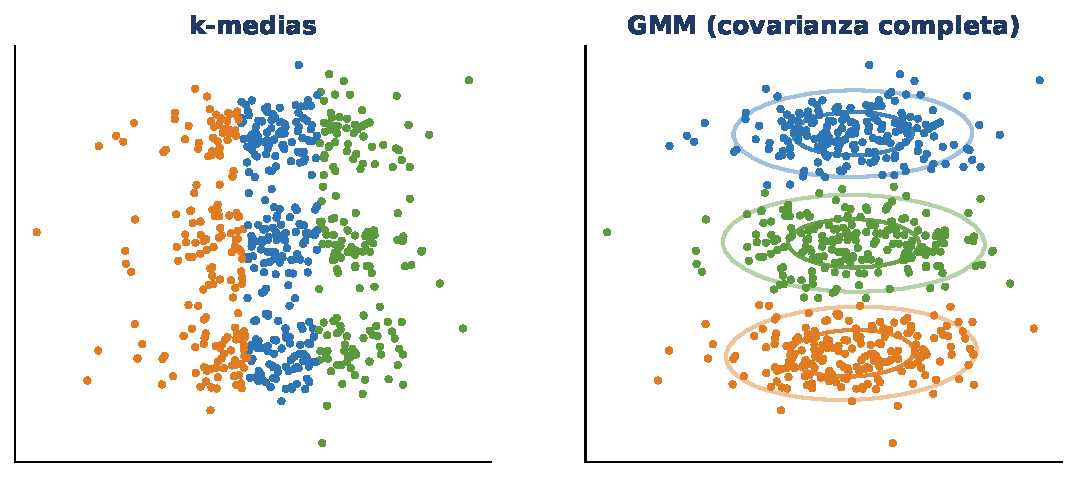
\includegraphics[width=0.72\textwidth]{gmm_vs_kmeans}
  \begin{itemize}
    \item Tres grupos alargados y paralelos: k-medias los corta en franjas verticales.
    \item GMM con covarianza completa recupera los grupos (elipses: 1 y 2 desviaciones).
  \end{itemize}
\end{frame}

\begin{frame}{Responsabilidades}
  \begin{columns}[c]
    \column{0.52\textwidth}
    Por el teorema de Bayes, la probabilidad de que $\x_i$ venga del componente $j$ es
    \[
      \gamma_{ij} = P(z_i=j\mid\x_i)
      = \frac{\pi_j\,\N(\x_i\mid\muv_j,\bm{\Sigma}_j)}{\sum_{l=1}^{k}\pi_l\,\N(\x_i\mid\muv_l,\bm{\Sigma}_l)} .
    \]
    \begin{itemize}
      \item $\gamma_{ij}$ se llama \alert{responsabilidad}.
      \item Asignación dura: $z_i = \arg\max_j \gamma_{ij}$.
      \item Los puntos en la frontera tienen responsabilidades cercanas a 0.5: la incertidumbre es información útil.
    \end{itemize}
    \column{0.45\textwidth}
    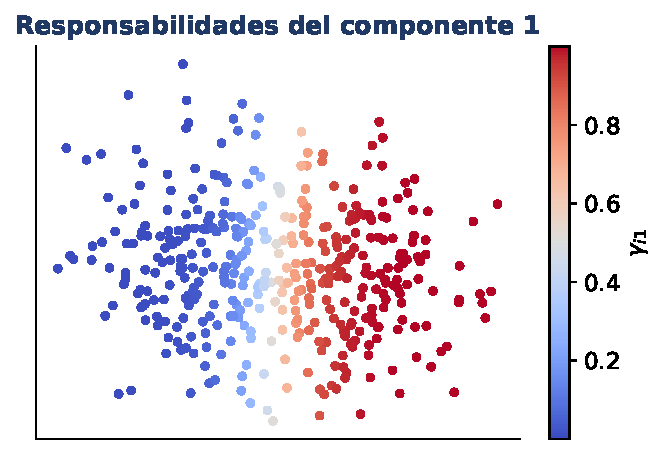
\includegraphics[width=\textwidth]{asignacion_suave}
  \end{columns}
\end{frame}

\begin{frame}{Máxima verosimilitud}
  Log-verosimilitud de los datos:
  \[
    \log L(\bm\theta) = \sum_{i=1}^{n}\log\Bigl(\sum_{j=1}^{k}\pi_j\,\N(\x_i\mid\muv_j,\bm{\Sigma}_j)\Bigr).
  \]
  \begin{itemize}
    \item El logaritmo de una suma no tiene solución cerrada.
    \item Si conociéramos $z_i$, el problema sería fácil: estimar una gaussiana por grupo.
    \item Singularidades: si un componente colapsa sobre un punto ($\bm{\Sigma}_j\to 0$), $\log L\to\infty$.
          Se evita con regularización (\texttt{reg\_covar}).
  \end{itemize}
  \begin{block}{Solución}
    El algoritmo de \textbf{esperanza-maximización (EM)}: alternar entre estimar las $z_i$
    (en forma suave) y reestimar los parámetros.
  \end{block}
\end{frame}

\begin{frame}{Algoritmo EM para GMM}
  Inicializar $\pi_j,\muv_j,\bm{\Sigma}_j$ y repetir hasta que $\log L$ deje de aumentar:
  \begin{block}{Paso E: calcular responsabilidades}
    \[
      \gamma_{ij} \leftarrow \frac{\pi_j\,\N(\x_i\mid\muv_j,\bm{\Sigma}_j)}{\sum_l \pi_l\,\N(\x_i\mid\muv_l,\bm{\Sigma}_l)}
    \]
  \end{block}
  \begin{block}{Paso M: reestimar parámetros, con $n_j = \sum_i \gamma_{ij}$}
    \[
      \muv_j \leftarrow \frac{1}{n_j}\sum_i \gamma_{ij}\,\x_i,\qquad
      \bm{\Sigma}_j \leftarrow \frac{1}{n_j}\sum_i \gamma_{ij}(\x_i-\muv_j)(\x_i-\muv_j)^\top,\qquad
      \pi_j \leftarrow \frac{n_j}{n}
    \]
  \end{block}
  {\small Cada iteración no disminuye $\log L$; converge a un máximo local.}
\end{frame}

\begin{frame}{EM y k-medias}
  \begin{itemize}
    \item k-medias es un caso límite de EM: covarianzas $\bm{\Sigma}_j = \varepsilon\mathbf{I}$
          con $\varepsilon\to 0$ y pesos iguales; las responsabilidades se vuelven 0 o 1.
    \item Paso E $\leftrightarrow$ asignación; paso M $\leftrightarrow$ actualización de centros.
  \end{itemize}
  \vspace{4pt}
  \begin{alertblock}{La inicialización también importa en EM}
    \begin{itemize}
      \item Por defecto, scikit-learn inicializa con k-medias: si k-medias falla, EM puede heredar el error.
      \item En la figura de GMM se usó \texttt{init\_params="random\_from\_data"} con \texttt{n\_init=10};
            con la inicialización por defecto, GMM también cortaba mal los grupos.
      \item Recomendación: varios reinicios y comparar la log-verosimilitud final.
    \end{itemize}
  \end{alertblock}
\end{frame}

\begin{frame}{Tipos de matriz de covarianza}
  \centering
  \renewcommand{\arraystretch}{1.35}
  \begin{tabular}{@{}llll@{}}
    \toprule
    \texttt{covariance\_type} & \textbf{Forma} & \textbf{Parámetros por componente} & \textbf{Grupos}\\
    \midrule
    \texttt{spherical} & $\sigma_j^2\mathbf{I}$ & $1$ & Esféricos, tamaño propio \\
    \texttt{diag}      & $\operatorname{diag}(\sigma_{j1}^2,\dots,\sigma_{jd}^2)$ & $d$ & Elipses alineadas a los ejes \\
    \texttt{tied}      & $\bm{\Sigma}$ compartida & $d(d+1)/2$ en total & Misma forma y orientación \\
    \texttt{full}      & $\bm{\Sigma}_j$ libre & $d(d+1)/2$ & Elipses arbitrarias \\
    \bottomrule
  \end{tabular}
  \vspace{8pt}
  \begin{itemize}
    \item Más flexibilidad requiere más datos: con $d$ grande, \texttt{full} puede sobreajustar.
    \item Es un hiperparámetro que se elige junto con $k$.
  \end{itemize}
\end{frame}

\begin{frame}{Selección de modelo: BIC y AIC}
  \begin{columns}[c]
    \column{0.5\textwidth}
    Con $p$ parámetros libres y $\hat L$ la verosimilitud máxima:
    \[
      \mathrm{BIC} = -2\log\hat L + p\log n, \qquad
      \mathrm{AIC} = -2\log\hat L + 2p .
    \]
    \begin{itemize}
      \item Ambos penalizan la complejidad; \textbf{menor es mejor}.
      \item BIC penaliza más y tiende a elegir modelos más simples.
      \item Se compara una rejilla de $k$ y \texttt{covariance\_type}.
    \end{itemize}
    \column{0.48\textwidth}
    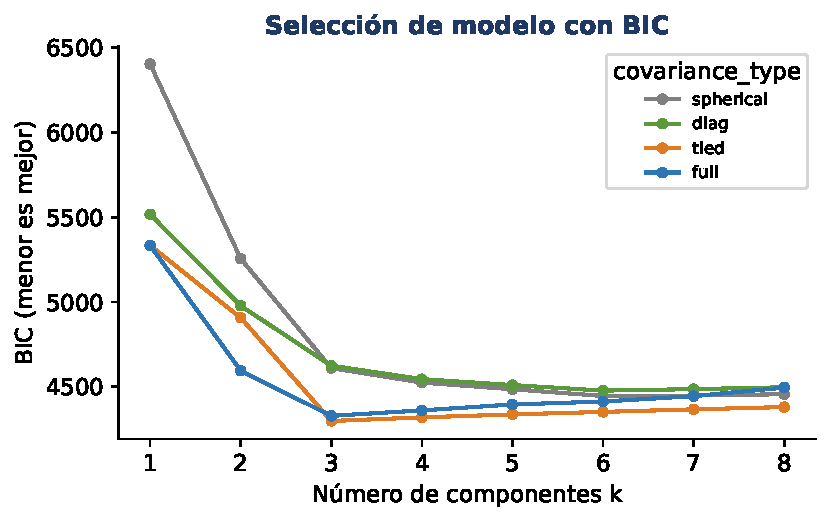
\includegraphics[width=\textwidth]{gmm_bic}
  \end{columns}
\end{frame}

\begin{frame}[fragile]{Laboratorio S4: GMM con scikit-learn}
\begin{lstlisting}
import numpy as np
from sklearn.mixture import GaussianMixture

resultados = []
for tipo in ["spherical", "diag", "tied", "full"]:
    for k in range(1, 9):
        gmm = GaussianMixture(k, covariance_type=tipo, n_init=5, random_state=0).fit(X)
        resultados.append((gmm.bic(X), k, tipo))
bic, k, tipo = min(resultados)
print("Mejor modelo:", k, tipo)

gmm = GaussianMixture(k, covariance_type=tipo, n_init=10,
                      init_params="random_from_data", random_state=0).fit(X)
z = gmm.predict(X)                  # asignacion dura
gamma = gmm.predict_proba(X)        # responsabilidades (n x k)
inciertos = np.sort(gamma, axis=1)[:, -1] < 0.6   # puntos sin grupo claro
log_dens = gmm.score_samples(X)     # log p(x): util para anomalias (Unidad 3)
\end{lstlisting}
  {\small Ejercicio: comparar GMM y k-medias en datos con grupos elípticos, con distintas inicializaciones.}
\end{frame}

% =====================================================================
\section{Sesión 5: Agrupamiento por densidad y espectral}
% =====================================================================

\begin{frame}{Grupos como regiones densas}
  \begin{itemize}
    \item Un grupo es una región de \alert{alta densidad} separada de otras por regiones de baja densidad.
    \item Permite formas arbitrarias (no convexas).
    \item No hay que fijar $k$.
    \item Los puntos en regiones poco densas se declaran \alert{ruido}: no se fuerza su asignación.
  \end{itemize}
  \vspace{6pt}
  \begin{block}{Algoritmos de esta sesión}
    \textbf{DBSCAN} (Ester et al., 1996), \textbf{OPTICS} (Ankerst et al., 1999) y
    \textbf{HDBSCAN} (Campello et al., 2013). Después, el \textbf{agrupamiento espectral},
    que ve los datos como un grafo.
  \end{block}
\end{frame}

\begin{frame}{DBSCAN}
  \begin{columns}[c]
    \column{0.5\textwidth}
    Parámetros: radio $\varepsilon$ y \texttt{min\_samples} $m$.
    \begin{itemize}
      \item $N_\varepsilon(\x) = \{\x' : d(\x,\x')\le\varepsilon\}$.
      \item \textbf{Núcleo}: $|N_\varepsilon(\x)|\ge m$ (incluye al propio punto).
      \item \textbf{Frontera}: no es núcleo, pero está en la vecindad de un núcleo.
      \item \textbf{Ruido}: ni núcleo ni frontera.
    \end{itemize}
    Un grupo = núcleos conectados por vecindades, más sus puntos frontera.
    \column{0.48\textwidth}
    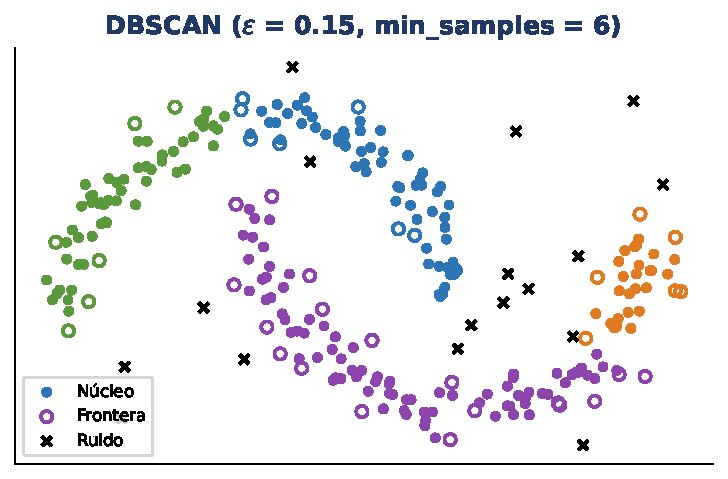
\includegraphics[width=\textwidth]{dbscan_tipos}
  \end{columns}
\end{frame}

\begin{frame}{Elección de parámetros en DBSCAN}
  \begin{columns}[c]
    \column{0.5\textwidth}
    \begin{itemize}
      \item \texttt{min\_samples}: regla práctica $m\ge d+1$; con ruido, $m\approx 2d$.
      \item $\varepsilon$: \textbf{gráfico de k-distancia} con $k=m$: ordenar la distancia de cada punto
            a su $k$-ésimo vecino y buscar el codo.
      \item Estandarizar antes: $\varepsilon$ es una distancia.
    \end{itemize}
    \begin{alertblock}{Limitaciones}
      \begin{itemize}
        \item Un solo $\varepsilon$ no sirve si los grupos tienen \alert{densidades distintas}.
        \item Sufre en alta dimensión (concentración de distancias).
      \end{itemize}
    \end{alertblock}
    \column{0.48\textwidth}
    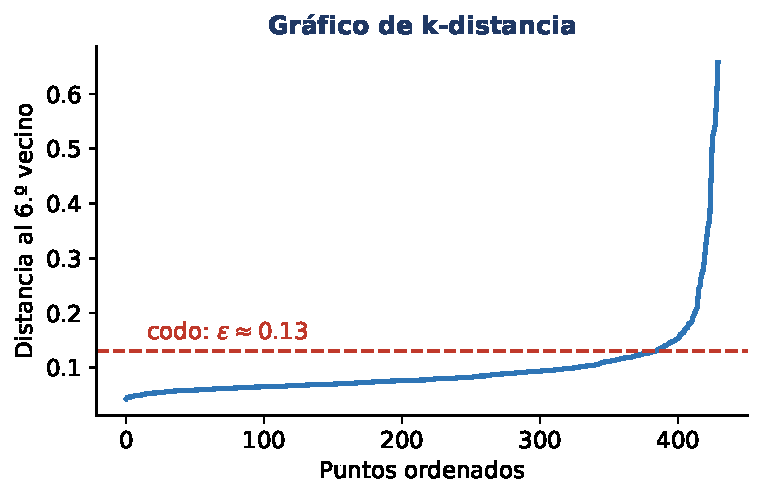
\includegraphics[width=\textwidth]{k_distancia}
  \end{columns}
\end{frame}

\begin{frame}{OPTICS y HDBSCAN}
  \textbf{Distancia núcleo} $\mathrm{core}_m(\x)$: distancia al $m$-ésimo vecino.
  \textbf{Distancia de alcanzabilidad mutua}:
  \[
    d_{\mathrm{mr}}(\bm{a},\bm{b}) = \max\{\mathrm{core}_m(\bm{a}),\ \mathrm{core}_m(\bm{b}),\ d(\bm{a},\bm{b})\}.
  \]
  \begin{columns}[T]
    \column{0.48\textwidth}
    \begin{block}{OPTICS}
      Ordena los puntos y produce un \textbf{gráfico de alcanzabilidad}: los valles son grupos.
      Equivale a correr DBSCAN para todos los $\varepsilon$ a la vez.
    \end{block}
    \column{0.48\textwidth}
    \begin{block}{HDBSCAN}
      \begin{enumerate}
        \item Árbol de expansión mínima con $d_{\mathrm{mr}}$.
        \item Jerarquía de grupos al variar el umbral.
        \item Árbol condensado con \texttt{min\_cluster\_size}.
        \item Elige los grupos más \alert{estables}.
      \end{enumerate}
    \end{block}
  \end{columns}
  \vspace{4pt}
  {\small HDBSCAN maneja densidades variables y casi no requiere ajustar $\varepsilon$.}
\end{frame}

\begin{frame}{Agrupamiento espectral: el grafo de similitud}
  \begin{enumerate}
    \item Construir un grafo con pesos $W_{ij}$:
          \begin{itemize}
            \item kernel gaussiano $W_{ij} = \exp(-\lVert\x_i-\x_j\rVert^2/2\sigma^2)$, o
            \item grafo de $k$ vecinos más cercanos (simetrizado).
          \end{itemize}
    \item Matriz de grados $\mathbf{D} = \operatorname{diag}(d_1,\dots,d_n)$, con $d_i = \sum_j W_{ij}$.
    \item Laplaciano del grafo:
          \[
            \mathbf{L} = \mathbf{D} - \mathbf{W},
            \qquad
            \mathbf{L}_{\mathrm{sym}} = \mathbf{I} - \mathbf{D}^{-1/2}\mathbf{W}\mathbf{D}^{-1/2}.
          \]
  \end{enumerate}
  \begin{block}{Propiedad clave}
    $\mathbf{L}$ es semidefinida positiva y la multiplicidad del eigenvalor 0 es el
    \textbf{número de componentes conexas} del grafo.
  \end{block}
\end{frame}

\begin{frame}{Agrupamiento espectral: algoritmo}
  \begin{columns}[c]
    \column{0.45\textwidth}
    Algoritmo de Ng, Jordan y Weiss (2002):
    \begin{enumerate}
      \item Calcular los $k$ eigenvectores de $\mathbf{L}_{\mathrm{sym}}$ con menores eigenvalores.
      \item Formar $\mathbf{U}\in\R^{n\times k}$ y normalizar sus filas.
      \item Aplicar k-medias a las filas de $\mathbf{U}$.
    \end{enumerate}
    \vspace{4pt}
    {\small Es una relajación del problema de \textbf{corte normalizado} del grafo.
    Costo: eigendescomposición, hasta $O(n^3)$.}
    \column{0.53\textwidth}
    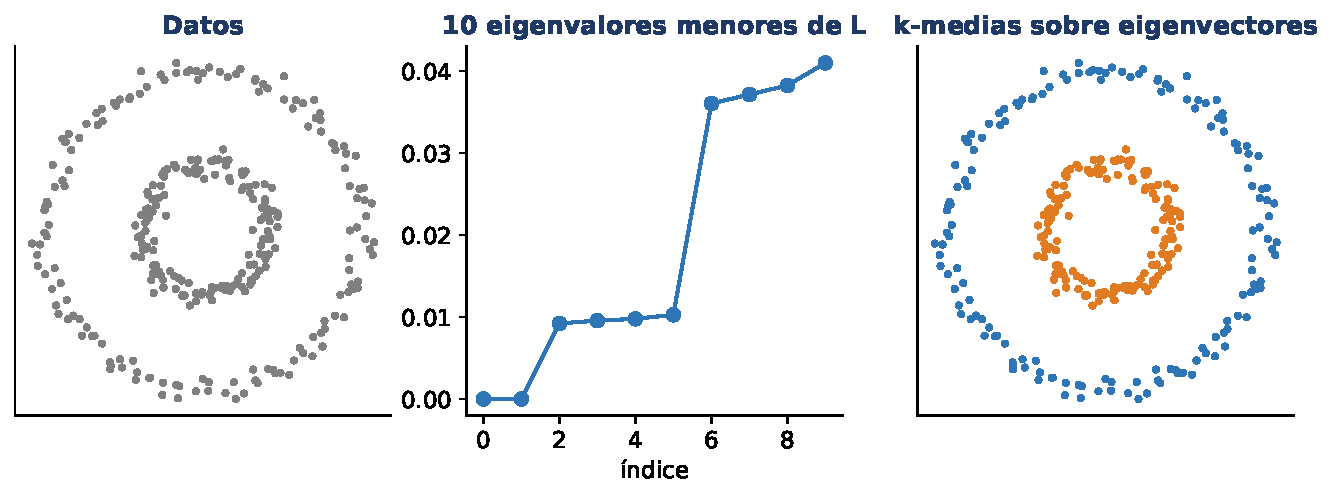
\includegraphics[width=\textwidth]{espectral_eigen}\\
    {\scriptsize Dos eigenvalores cercanos a cero: dos componentes casi desconectadas.}
  \end{columns}
\end{frame}

\begin{frame}{Comparación en formas difíciles}
  \centering
  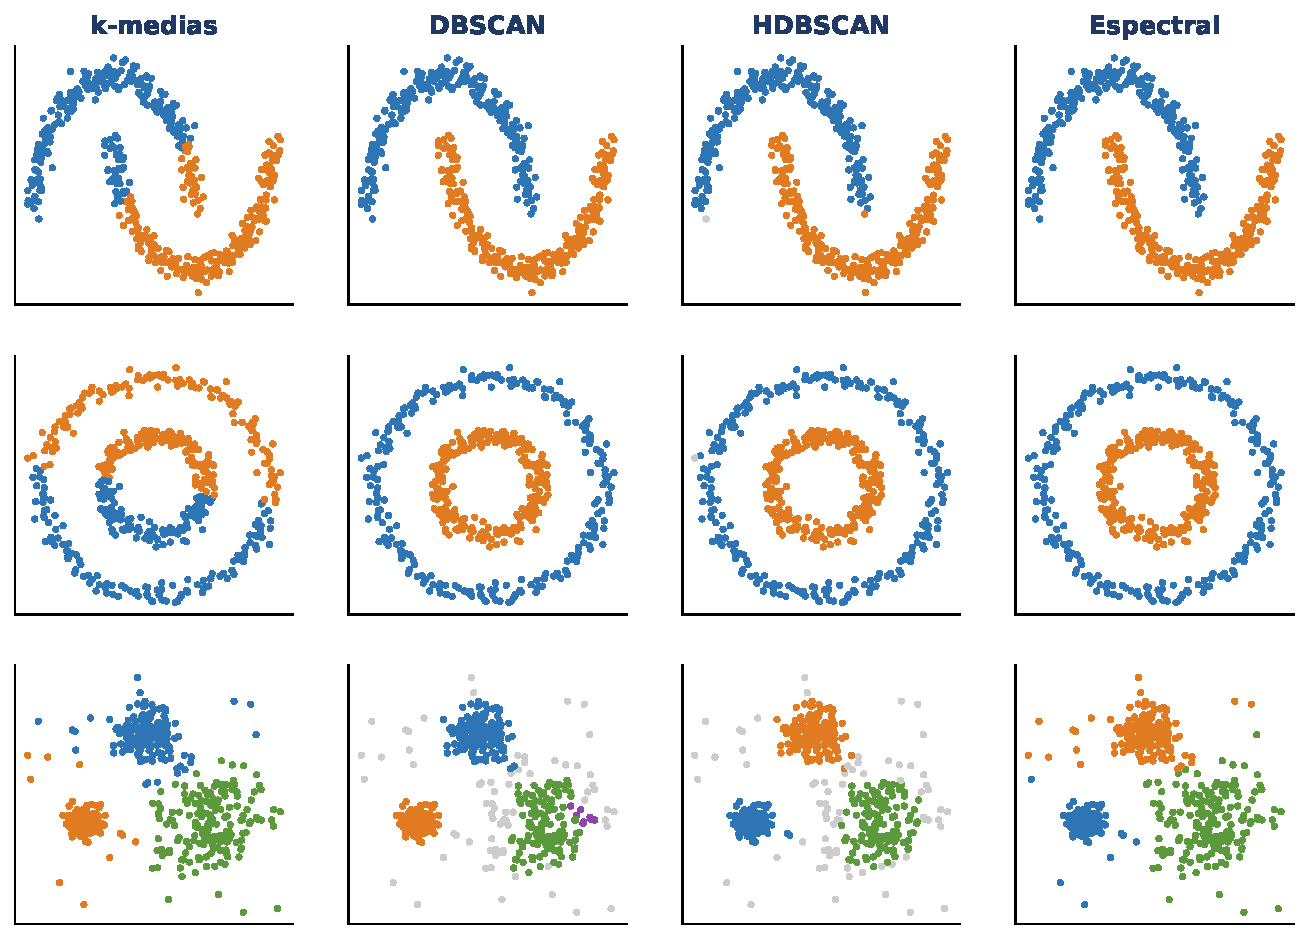
\includegraphics[height=0.74\textheight]{comparacion_densidad}\\
  {\small Datos estandarizados. Gris: puntos marcados como ruido. Fila 3: densidades distintas con ruido de fondo.}
\end{frame}

\begin{frame}[fragile]{Laboratorio S5: densidad y espectral}
\begin{lstlisting}
import numpy as np
from sklearn.datasets import make_moons
from sklearn.preprocessing import StandardScaler
from sklearn.neighbors import NearestNeighbors
from sklearn.cluster import DBSCAN, HDBSCAN, SpectralClustering

X, y = make_moons(500, noise=0.06, random_state=0)
X = StandardScaler().fit_transform(X)

m = 8
d, _ = NearestNeighbors(n_neighbors=m).fit(X).kneighbors(X)
k_dist = np.sort(d[:, -1])                    # graficar y buscar el codo -> eps

db = DBSCAN(eps=0.25, min_samples=m).fit(X)
print("grupos:", len(set(db.labels_) - {-1}), "ruido:", np.sum(db.labels_ == -1))

hdb = HDBSCAN(min_cluster_size=20).fit(X)     # scikit-learn >= 1.3
prob = hdb.probabilities_                     # fuerza de pertenencia

esp = SpectralClustering(2, affinity="nearest_neighbors", n_neighbors=10,
                         random_state=0).fit(X)
\end{lstlisting}
\end{frame}

% =====================================================================
\section{Sesión 6: Validación e interpretación}
% =====================================================================

\begin{frame}{¿Cómo saber si un agrupamiento es bueno?}
  \begin{itemize}
    \item \textbf{Validación interna}: sólo usa los datos y las etiquetas encontradas (compacidad y separación).
    \item \textbf{Validación externa}: compara con una etiqueta de referencia, si existe.
    \item \textbf{Estabilidad}: ¿los grupos se repiten al perturbar los datos?
    \item \textbf{Utilidad}: ¿los grupos tienen sentido y sirven para decidir?
  \end{itemize}
  \vspace{6pt}
  \begin{alertblock}{Cuidado}
    Todo algoritmo encuentra grupos, incluso en datos sin estructura. Y cada índice interno
    favorece a cierto tipo de grupos: la silueta favorece grupos convexos, como k-medias.
  \end{alertblock}
\end{frame}

\begin{frame}{Diagrama de silueta}
  \centering
  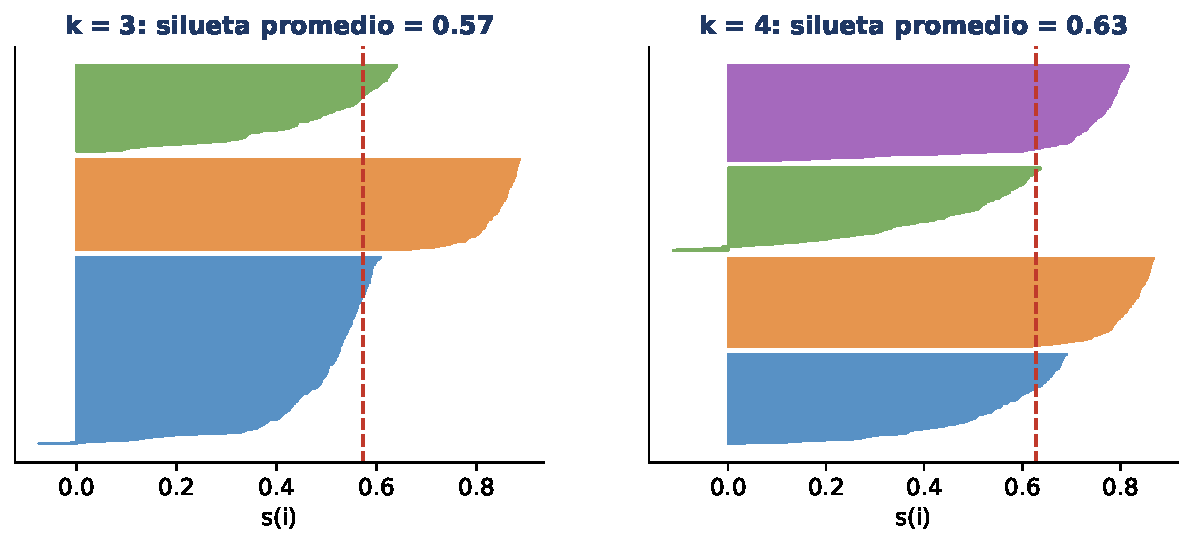
\includegraphics[width=0.8\textwidth]{diagrama_silueta}
  \begin{itemize}
    \item Cada barra es un punto; cada color, un grupo.
    \item Valores negativos: puntos probablemente mal asignados.
    \item Además del promedio, revisar que todos los grupos superen la media y tengan grosor parecido.
  \end{itemize}
\end{frame}

\begin{frame}{Índices internos}
  \centering
  \renewcommand{\arraystretch}{1.12}
  \begin{tabular}{@{}lll@{}}
    \toprule
    \textbf{Índice} & \textbf{Definición} & \textbf{Mejor}\\
    \midrule
    Silueta & $\dfrac{1}{n}\sum_i \dfrac{b(i)-a(i)}{\max\{a(i),b(i)\}}$ & Mayor (máx.\ 1) \\
    Davies-Bouldin & $\dfrac{1}{k}\sum_{j}\max_{l\neq j}\dfrac{s_j+s_l}{\lVert\muv_j-\muv_l\rVert}$ & Menor (mín.\ 0) \\
    Calinski-Harabasz & $\dfrac{\operatorname{tr}(\mathbf{B})/(k-1)}{\operatorname{tr}(\mathbf{W})/(n-k)}$ & Mayor \\
    \bottomrule
  \end{tabular}\par
  \vspace{2pt}
  {\scriptsize $s_j$: distancia media de los puntos del grupo $j$ a su centro.
  $\mathbf{B}$, $\mathbf{W}$: matrices de dispersión entre grupos y dentro de los grupos.}\par
  \vspace{2pt}
  \centering
  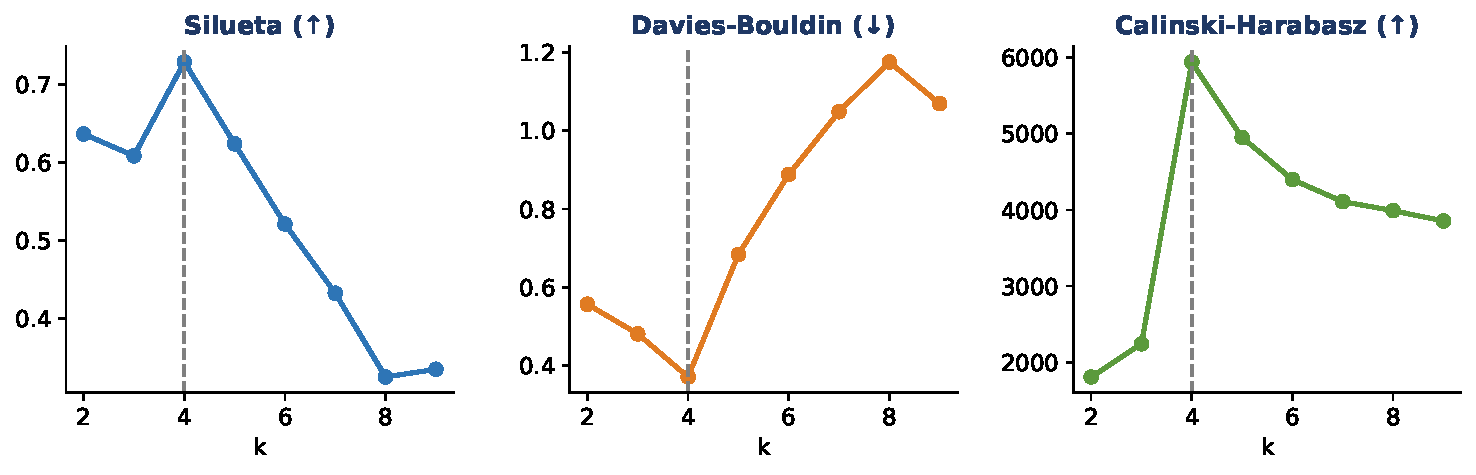
\includegraphics[width=0.62\textwidth]{indices_internos}
\end{frame}

\begin{frame}{Índices externos}
  Cuando existe una etiqueta de referencia $y$ (para evaluar métodos, no para entrenarlos):
  \vspace{4pt}
  \begin{itemize}
    \item \textbf{Índice de Rand ajustado (ARI)}: proporción de pares de puntos en los que ambas
          particiones coinciden (juntos o separados), corregida por azar.
          Vale 1 si son idénticas y $\approx 0$ si la coincidencia es aleatoria.
    \item \textbf{Información mutua normalizada (NMI)}:
          \[
            \mathrm{NMI}(Y,Z) = \frac{I(Y;Z)}{\tfrac{1}{2}\left[H(Y)+H(Z)\right]}\in[0,1].
          \]
  \end{itemize}
  \begin{block}{Propiedades}
    Ambos son invariantes a permutar los nombres de los grupos y admiten distinto número
    de grupos en cada partición.
  \end{block}
\end{frame}

\begin{frame}{Estabilidad}
  \begin{columns}[c]
    \column{0.55\textwidth}
    \begin{enumerate}
      \item Tomar $B$ submuestras (o muestras bootstrap) de los datos.
      \item Agrupar cada una con el mismo algoritmo y parámetros.
      \item Comparar las particiones en los puntos comunes con ARI.
      \item Promediar: valores altos indican grupos estables.
    \end{enumerate}
    \vspace{4pt}
    {\small También sirve para elegir $k$: preferir el $k$ más estable.}
    \column{0.42\textwidth}
    \centering
    \begin{tikzpicture}[node distance=6mm]
      \node[caja] (d) {Datos};
      \node[caja,below left=6mm and 2mm of d] (m1) {Submuestra 1};
      \node[caja,below right=6mm and 2mm of d] (m2) {Submuestra 2};
      \node[caja,below=6mm of m1] (z1) {Partición 1};
      \node[caja,below=6mm of m2] (z2) {Partición 2};
      \node[caja,fill=naranja!15,draw=naranja] (a) at ($(z1)!0.5!(z2)+(0,-1.4)$) {ARI en puntos comunes};
      \draw[flecha] (d) -- (m1); \draw[flecha] (d) -- (m2);
      \draw[flecha] (m1) -- (z1); \draw[flecha] (m2) -- (z2);
      \draw[flecha] (z1) -- (a); \draw[flecha] (z2) -- (a);
    \end{tikzpicture}
  \end{columns}
\end{frame}

\begin{frame}{Interpretación y comunicación}
  \begin{itemize}
    \item \textbf{Perfilar} cada grupo: tamaño, medias o medianas de las variables originales (no estandarizadas).
    \item Comparar cada grupo contra el total: ¿qué variables lo distinguen?
    \item Un \textbf{árbol de decisión} entrenado para predecir el grupo da reglas legibles.
    \item Visualizar con PCA o t-SNE (Unidad 2), sin sobreinterpretar.
    \item Ponerle \textbf{nombre} a cada grupo con ayuda de expertos del dominio.
  \end{itemize}
  \vspace{4pt}
  \begin{alertblock}{Impacto en decisiones}
    Un segmento puede convertirse en una política o un programa. Revisar si los grupos
    reproducen sesgos (por ejemplo, por región o género) y documentar las decisiones del análisis.
  \end{alertblock}
\end{frame}

\begin{frame}[fragile]{Laboratorio S6: validación}
\begin{lstlisting}[basicstyle=\ttfamily\fontsize{6.5}{7.5}\selectfont]
import numpy as np
from sklearn.cluster import KMeans
from sklearn.metrics import (silhouette_score, davies_bouldin_score,
    calinski_harabasz_score, adjusted_rand_score, normalized_mutual_info_score)

def estabilidad(X, k, B=20, frac=0.8, semilla=0):
    rng = np.random.default_rng(semilla)
    n, aris = len(X), []
    for b in range(B):
        i1 = rng.choice(n, int(frac * n), replace=False)
        i2 = rng.choice(n, int(frac * n), replace=False)
        comunes = np.intersect1d(i1, i2)
        m1 = KMeans(k, n_init=10, random_state=b).fit(X[i1])
        m2 = KMeans(k, n_init=10, random_state=b + B).fit(X[i2])
        aris.append(adjusted_rand_score(m1.predict(X[comunes]), m2.predict(X[comunes])))
    return np.mean(aris)

for k in range(2, 9):
    z = KMeans(k, n_init=10, random_state=0).fit_predict(X)
    print(k, silhouette_score(X, z), davies_bouldin_score(X, z),
          calinski_harabasz_score(X, z), estabilidad(X, k))
# Si hay etiqueta de referencia y: adjusted_rand_score(y, z), normalized_mutual_info_score(y, z)
\end{lstlisting}
\end{frame}

% =====================================================================
\section{Cierre de la unidad}
% =====================================================================

\begin{frame}{¿Qué algoritmo elegir?}
  \centering
  \begin{tikzpicture}[
      q/.style={draw=marino,fill=azul!10,rounded corners,align=center,font=\small,minimum height=8mm},
      r/.style={draw=naranja,fill=naranja!12,rounded corners,align=center,font=\small,minimum height=7mm},
      lab/.style={font=\scriptsize,midway,fill=white,inner sep=1pt},
      >={Stealth}]
    \node[q] (q1) at (0,0) {¿Se espera ruido o formas arbitrarias?};
    \node[q] (q2) at (-4,-1.7) {¿Interesa la jerarquía?};
    \node[q] (q3) at (4,-1.7) {¿Densidades distintas?};
    \node[q] (q4) at (-5.6,-3.4) {¿Grupos elípticos o\\asignación suave?};
    \node[r] (r1) at (-1.8,-3.4) {Jerárquico\\(elegir enlace)};
    \node[r] (r2) at (-7,-5.1) {GMM};
    \node[r] (r3) at (-4.2,-5.1) {k-medias};
    \node[r] (r4) at (2.6,-3.4) {DBSCAN};
    \node[r] (r5) at (5.6,-3.4) {HDBSCAN};
    \node[r] (r6) at (4,-5.1) {Espectral (si se conoce $k$)};
    \draw[->,thick,marino] (q1) -- node[lab]{no} (q2);
    \draw[->,thick,marino] (q1) -- node[lab]{sí} (q3);
    \draw[->,thick,marino] (q2) -- node[lab]{no} (q4);
    \draw[->,thick,marino] (q2) -- node[lab]{sí} (r1);
    \draw[->,thick,marino] (q4) -- node[lab]{sí} (r2);
    \draw[->,thick,marino] (q4) -- node[lab]{no} (r3);
    \draw[->,thick,marino] (q3) -- node[lab]{no} (r4);
    \draw[->,thick,marino] (q3) -- node[lab]{sí} (r5);
    \draw[->,thick,marino,dashed] (q3) -- node[lab]{sin ruido} (r6);
  \end{tikzpicture}
\end{frame}

\begin{frame}{Resumen}
  \renewcommand{\arraystretch}{1.2}
  \small
  \centering
  \begin{tabular}{@{}lccccc@{}}
    \toprule
    & \textbf{Fijar $k$} & \textbf{Formas} & \textbf{Ruido} & \textbf{Escala a $n$ grande} & \textbf{Salida}\\
    \midrule
    k-medias      & sí & esféricas & no & sí & partición \\
    Jerárquico    & al cortar & según enlace & no & no & árbol \\
    GMM           & sí & elípticas & no & sí & probabilidades \\
    DBSCAN        & no & arbitrarias & sí & sí & partición + ruido \\
    HDBSCAN       & no & arbitrarias & sí & sí & partición + ruido \\
    Espectral     & sí & arbitrarias & no & no & partición \\
    \bottomrule
  \end{tabular}
  \vspace{8pt}
  \begin{block}{Ideas clave}
    Preprocesar con cuidado; probar varios algoritmos; validar con índices, estabilidad y
    criterio experto; describir los grupos en términos del problema.
  \end{block}
\end{frame}

\begin{frame}{Miniproyecto 1: algoritmos de agrupamiento}
  \begin{columns}[T]
    \column{0.55\textwidth}
    \begin{block}{Encargo}
      Elegir un conjunto de datos real de un sector productivo o social y:
      \begin{enumerate}
        \item Preparar los datos y justificar la escala y la distancia.
        \item Aplicar al menos tres familias de algoritmos.
        \item Elegir hiperparámetros con índices internos y estabilidad.
        \item Perfilar e interpretar los grupos finales.
        \item Discutir qué decisiones informan y sus posibles sesgos.
      \end{enumerate}
    \end{block}
    \column{0.41\textwidth}
    \begin{exampleblock}{Entrega (S6)}
      \begin{itemize}
        \item Notebook reproducible
        \item Informe breve con la interpretación
        \item Peso: 30\,\% de la calificación
      \end{itemize}
    \end{exampleblock}
    \begin{alertblock}{Pregunta guía}
      ¿Cómo convencerías a alguien sin formación técnica de que tus grupos son reales y útiles?
    \end{alertblock}
  \end{columns}
\end{frame}

\begin{frame}{Lecturas de la unidad}
  \begin{itemize}
    \item James, G., Witten, D., Hastie, T., Tibshirani, R. y Taylor, J. (2023).
          \emph{An Introduction to Statistical Learning with Applications in Python}.
          Springer. \alert{Cap.~12.4: Clustering Methods} (k-medias y jerárquico).
    \item Bishop, C.\,M. (2006). \emph{Pattern Recognition and Machine Learning}.
          Springer. \alert{Cap.~9: Mixture Models and EM} (k-medias, GMM, EM).
    \item Murphy, K.\,P. (2022). \emph{Probabilistic Machine Learning: An Introduction}.
          MIT Press. \alert{Cap.~21: Clustering} (evaluación, jerárquico, k-medias, mezclas, espectral).
    \item Hinton, G.\,E. y Sejnowski, T.\,J. (Eds.) (1999). \emph{Unsupervised Learning:
          Foundations of Neural Computation}. MIT Press. (Complementaria.)
  \end{itemize}
  \vspace{4pt}
  {\small Artículos originales: Arthur y Vassilvitskii (2007), k-means++; Ester et al.\ (1996), DBSCAN;
  Campello, Moulavi y Sander (2013), HDBSCAN; Ng, Jordan y Weiss (2002), agrupamiento espectral;
  von Luxburg (2007), tutorial de agrupamiento espectral; Rousseeuw (1987), silueta.}
\end{frame}

\end{document}
